% !TeX root = ../thuthesis-example.tex

\chapter{集群故障检测}

本章节描述了高可用优化下的集群错误检测机制。ConfigNode Leader 是集群故障检测的负责人。ConfigNode Leader通过维护和DataNode之间定期心跳的方式来获取每个节点的基本负载情况、Region负载情况等信息,通过定期要求DataNode之间进行P2P探测的方式来获取集群的网络拓扑结构。同时,我们使用了基于Phi Accural的检测算法对于收集到的探测包进行故障研判,并根据Thrift进行了一些优化。

\section{节点和Region的心跳机制}

IoTDB使用心跳机制来探测集群内部节点和每一个Region的健康状态,从而能够第一时间检测出集群内进程崩溃、网络分区的问题。

ConfigNode是集群的大脑,负责维护每一个节点的状态信息。在ConfigNode、DataNode和AINode启动的时候,都需要向ConfigNode的Leader汇报自己的启动信息,由ConfigNode Leader将其纳入心跳管理的范围内。当节点下线、被移出集群、重启时也会汇报最新的状态,让ConfigNode Leader知悉。

对于注册在集群的所有节点,ConfigNode会定期使用内部RPC向每一个节点发送心跳,来更新确认节点的最新状态。心跳会按照固定时间间隔触发,通常间隔是1s。
ConfigNode Leader会通过心跳向DataNode传输Quota和集群拓扑结构等信息,

DataNode会通过心跳上报当前的状态、节点的CPU、内存、磁盘的使用情况、每一个Region目前的Consensus的Leader分布、每一个Region的磁盘使用情况、日志同步情况、当前的Pipe任务情况等相关内容。


在收集到心跳样本之后,ConfigNode Leader会根据心跳样本的情况对集群的情况做出处理。

ConfigNode首先会对该节点本本身的状态进行研判。在2.0.2.1等先前版本中,如果在一个固定的超时间隔之内(通常是20s)都没有收到DataNode上报的心跳,那么ConfigNode Leader就会研判该节点已经失效,将该节点的状态从RUNNING标记为UNKNOWN。这种基于固定超时时间间隔的算法能够检测出大部分的实际问题,但依然有改进的空间,再下一个小节中我们通过提出基于PhiAccrual的方式对该研判方法进行升级。

ConfigNode其次会根据收集到的Load情况和每一个Region的情况进行相应的研判,从而做出预防性高可用的操作。例如负载均衡、Region迁移、磁盘告警等操作,从而减少错误的产生。


(这部分可以增加一张示意图来描述整一个过程)
(这部分可以详细描述预防性操作的一些行为)



\section{基于Phi Accrual的故障检测}

如前文所述,在2.0.2.1等先前版本之前,ConfigNode Leader采用基于心跳的固定超时来研判节点的存活情况。该算法研判的核心参数在于超时时间 $\Delta_{t}$,即当ConfigNode Leader在超过 $\Delta_{t}$ 的时间内没有收到DataNode的心跳包,则会认为该节点宕机。

参数 $\Delta_{t}$ 是故障检测的检测速度和检测正确度的权衡。如果 $\Delta_{t}$ 很短,那么节点故障会被快速发现,但对应的误报率就会很高。如果$\Delta_{t}$很长,那么误报率就会对应下降,但是代价就是错误的平均发现时间变长。

这种基于心跳的固定超时算法的优点在于逻辑简单直接,易于实现和部署,并且在IoTDB已有的实践中能胜任大部分的错误发现。然而这种算法依然存在诸多问题。
首先,$\Delta_{t}$ 参数的选择需要人工介入,需要对业务集群的特性有所了解,对很多用户来说是一个很大的心智负担。其次,$\Delta_{t}$ 参数一旦确定,轻易不能改变,这导致心跳算法无法对集群随时间的状态迁移作出适配。例如,集群流量如果有明显的时段性变化,那么显然在高负载时期和低负载时期都使用同一个参数并不明智。最后,该算法只能给出故障/正常的二元结论,无法给出量化的数据。

前文提出的Phi Accural算法有冷启动的问题。因此我们的故障检测综合

1. 冷启动阶段。在集群刚启动,尚未收集足够的心跳样本的时候,我们使用基于心跳的固定超时来负责初始时期的节点存活判断,同时收集这些样本。当我们收集了足够的样本数量(默认为60个)的时候,我们切换成基于Phi Accural的算法来研判节点的存活率。

1. 心跳历史样本收集。检测器会收集每一个DataNode心跳包,并计算出连续两个心跳包之间的间隔,并存储在一个固定大小的采样窗口内,当有新的心跳包到达的时候,最新的时间间隔会被存入采样窗口,而最早期的第一个数据将会被删除。

2. 根据采样窗口计算到达间隔的分布,并计算 $\phi$ 值。我们将到达间隔认为是符合正态分布。那么我们就可以从采样窗口来估计这个分布的均值 $\mu$ 和方差 $\sigma^2$。那么,在上一次心跳到达t时间之后才会有下一次心跳到达的概率可以通过下列公式计算出来:

$$ P_{later}(t) = \frac{1}{\sigma\sqrt{2\pi}} \int_{t}^{\infty} e^{-\frac{(x-u)^2}{2\sigma^2}} dx $$

3. 计算 $\phi$ 并根据设定阈值进行比较。我们使用如下的公式进行定义:

$$ \phi(now) = -log_{10}(P_{later}(t_{now} - t_{last})) $$

不同的阈值代表着本次研判出错的概率。阈值=1的时候研判出错的概率是10\%,阈值=1的时候研判出错的概率是1\%,阈值=3的时候研判出错的概率是0.1\%。

「在实验章节给出这两种故障检测算法的实验对比」

\section{集群网络拓扑感知}

上述所述的心跳和故障检测机制能够迅速识别集群中的节点宕机和对称性网络分区等问题,但针对非对称网络分区等问题依然无法识别。为此,我们需要在此基础上增加集群网络拓扑感知能力。

\begin{figure}
  \centering
  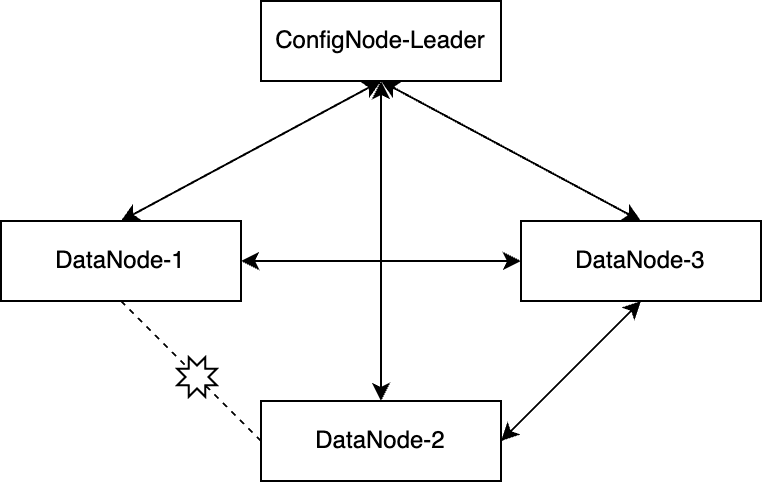
\includegraphics[width=0.9\linewidth]{c03-parition.png}
  \caption{系统非对称分区示意图}
  \label{fig:c03-partition}
\end{figure}

考虑图\ref{fig:c03-partition}所示的系统情况,集群由1个ConfigNode和3个DataNode组成,其中ConfigNode和所有三个DataNode都能正常了连接交换情况,但是DataNode1和DataNode2之间的网络连接可能因为配置不当或者线缆断裂而出现非对称网络分区。这种对称网络分区的问题不能被上述提到的心跳机制所捕捉,并且可能会产生严重的问题,例如:

1. 两副本模式下,如果同一个Region的两个副本分别处于DataNode1和DataNode2上,那么该Region在事实意义上属于不高可用的状态,需要ConfigNode触发对应的Region迁移等操作。
2. 如果客户端连接到了DataNode1上,但是写入请求需要被转发到DataNode2上,那么这次写入就会失败,相关数据有可能丢失。
3. 如果客户端的查询请求被调度了DataNode1上,并且查询请求的Root Fragment Instance被放置在DataNode2上,那么本次查询就没有办法获取所有的被查数据,从而失败。

为了解决这个问题,我们在客户端连接、查询规划、写入执行的时候都需要知道集群的整体拓扑情况,从而规避因为非对称分区而产生的请求问题。

\begin{figure}
  \centering
  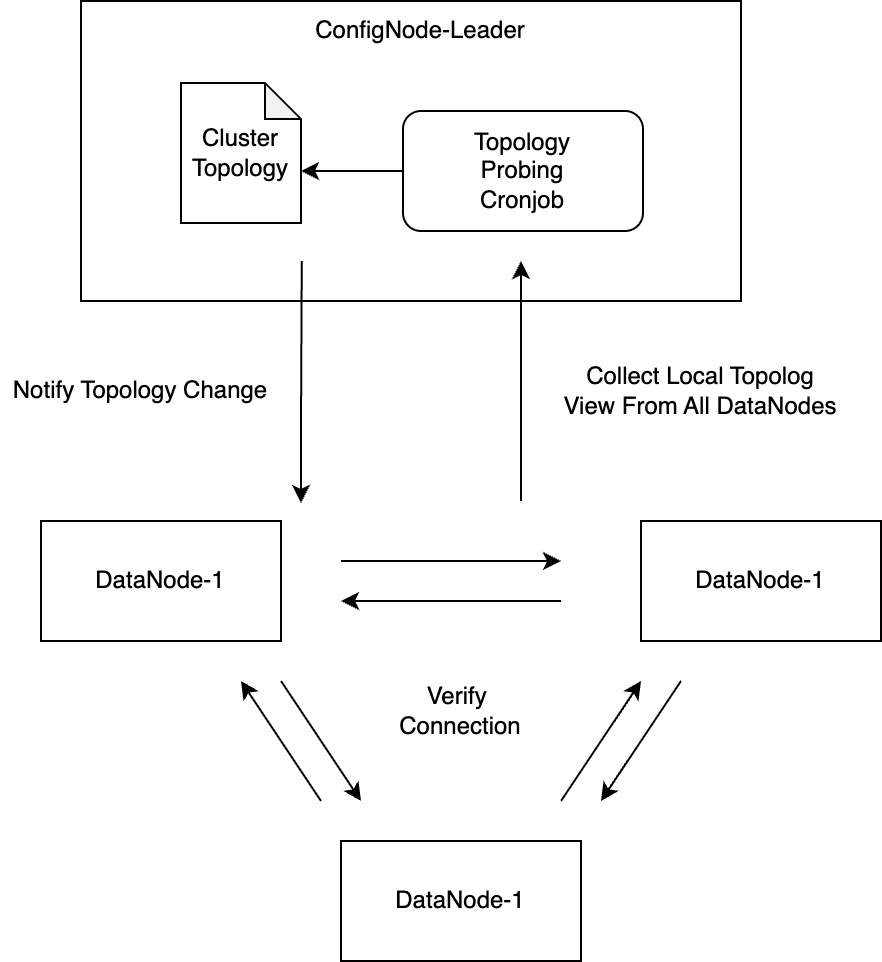
\includegraphics[width=0.7\linewidth]{c03-topology.png}
  \caption{集群拓扑感知能力}
  \label{fig:c03-topology}
\end{figure}

我们通过DataNode之间的P2P心跳来实现集群拓扑感知的功能。图\ref{fig:c03-topology}展示了集群拓扑感知的全流程。ConfigNode Leader会启动定期的任务,要求每一个DataNode需要向其他的所有DataNodes发送探测性质的RPC请求,来验证是否能够和所有DataNodes都完全联通,并在规定的时间内向ConfigNode上报本次的探测结果。

ConfigNode会收集所有DataNode的本地连通性,并同样维护一个固定大小的采样窗口。接着ConfigNode会使用上一小节中提到的Phi Accrual算法来判断DataNodes之间的两两连通性,最终获得全局拓扑图。
一旦ConfigNode发现全局拓扑图更新,那么就会在下一次和DataNode交换心跳包的时候将这个拓扑图给下发到每一个DataNode节点,使得每一个DataNode节点上都能够存储一份最新的集群视角的拓扑结构,用于后续的查询计划生成和写入请求。


\section{基于长期连接的优化}

在部分情况下,例如通过操作系统强制Kill一个IoTDB进程,我们可以通过特殊的机制进一步加快错误的发生,这是通过TCP信道来实现的。
IoTDB内部采用ClientManager接口来统一管理对外的Thrift连接。ClientManager的基本原理类似于带缓存的连接池。当我们首次请求某一个新的EndPoint的TCP连接请求,ClientManager会建立这个TCP连接。当我们结束使用的时候,ClientManager并不会直接将这个TCP连接断开,而是继续维持一段时间,并把连接缓存在本地。这样在下次我们需要请求相同的EndPoint地址的时候,我们就不需要负担重新建立TCP的开销,可以直接复用ClientManager内部缓存的连接。当我们长期不使用某一个TCP连接的时候,ClientManager就会销毁这个连接并且清理对应的资源。

由于ConfigNode和每一个DataNode之间都有大量的内部RPC交换,因此通过ClientManager的机制,我们可以认为ConfigNode和DataNode之间建立了一个长期有效的TCP连接信道。此时当该进程突然断开,那么Thrift就能够立马汇报信道的问题,这种汇报的时间延迟通常在一秒钟之内,非常快速,而不需要依赖上述所说的Phi Accural算法,后者的发现延迟通常在十秒之上。


(其实这里我觉得应该变成Thrift连接)




中文论文的数学符号默认遵循 GB/T 3102.11—1993《物理科学和技术中使用的数学符号》
\footnote{原 GB 3102.11—1993,自 2017 年 3 月 23 日起,该标准转为推荐性标准。}。
该标准参照采纳 ISO 31-11:1992 \footnote{目前已更新为 ISO 80000-2:2019。},
但是与 \TeX{} 默认的美国数学学会(AMS)的符号习惯有所区别。
具体地来说主要有以下差异:
\begin{enumerate}
  \item 大写希腊字母默认为斜体,如
    \begin{equation*}
      \Gamma \Delta \Theta \Lambda \Xi \Pi \Sigma \Upsilon \Phi \Psi \Omega.
    \end{equation*}
    注意有限增量符号 $\increment$ 固定使用正体,模板提供了 \cs{increment} 命令。
  \item 小于等于号和大于等于号使用倾斜的字形 $\le$、$\ge$。
  \item 积分号使用正体,比如 $\int$、$\oint$。
  \item
    偏微分符号 $\partial$ 使用正体。
  \item
    省略号 \cs{dots} 按照中文的习惯固定居中,比如
    \begin{equation*}
      1, 2, \dots, n \quad 1 + 2 + \dots + n.
    \end{equation*}
  \item
    实部 $\Re$ 和虚部 $\Im$ 的字体使用罗马体。
\end{enumerate}

以上数学符号样式的差异可以在模板中统一设置。
另外国标还有一些与 AMS 不同的符号使用习惯,需要用户在写作时进行处理:
\begin{enumerate}
  \item 数学常数和特殊函数名用正体,如
    \begin{equation*}
      \uppi = 3.14\dots; \quad
      \symup{i}^2 = -1; \quad
      \symup{e} = \lim_{n \to \infty} \left( 1 + \frac{1}{n} \right)^n.
    \end{equation*}
  \item 微分号使用正体,比如 $\dif y / \dif x$。
  \item 向量、矩阵和张量用粗斜体(\cs{symbf}),如 $\symbf{x}$、$\symbf{\Sigma}$、$\symbfsf{T}$。
  \item 自然对数用 $\ln x$ 不用 $\log x$。
\end{enumerate}


英文论文的数学符号使用 \TeX{} 默认的样式。
如果有必要,也可以通过设置 \verb|math-style| 选择数学符号样式。

关于量和单位推荐使用
\href{http://mirrors.ctan.org/macros/latex/contrib/siunitx/siunitx.pdf}{\pkg{siunitx}}
宏包,
可以方便地处理希腊字母以及数字与单位之间的空白,
比如:
\SI{6.4e6}{m},
\SI{9}{\micro\meter},
\si{kg.m.s^{-1}},
\SIrange{10}{20}{\degreeCelsius}。



\section{数学公式}

数学公式可以使用 \env{equation} 和 \env{equation*} 环境。
注意数学公式的引用应前后带括号,通常使用 \cs{eqref} 命令,比如式\eqref{eq:example}。
\begin{equation}
  \frac{1}{2 \uppi \symup{i}} \int_\gamma f = \sum_{k=1}^m n(\gamma; a_k) \mathscr{R}(f; a_k).
  \label{eq:example}
\end{equation}

多行公式尽可能在“=”处对齐,推荐使用 \env{align} 环境。
\begin{align}
  a & = b + c + d + e \\
    & = f + g
\end{align}



\section{数学定理}

定理环境的格式可以使用 \pkg{amsthm} 或者 \pkg{ntheorem} 宏包配置。
用户在导言区载入这两者之一后,模板会自动配置 \env{theorem}、\env{proof} 等环境。

\begin{theorem}[Lindeberg--Lévy 中心极限定理]
  设随机变量 $X_1, X_2, \dots, X_n$ 独立同分布, 且具有期望 $\mu$ 和有限的方差 $\sigma^2 \ne 0$,
  记 $\bar{X}_n = \frac{1}{n} \sum_{i+1}^n X_i$,则
  \begin{equation}
    \lim_{n \to \infty} P \left(\frac{\sqrt{n} \left( \bar{X}_n - \mu \right)}{\sigma} \le z \right) = \Phi(z),
  \end{equation}
  其中 $\Phi(z)$ 是标准正态分布的分布函数。
\end{theorem}
\begin{proof}
  Trivial.
\end{proof}

同时模板还提供了 \env{assumption}、\env{definition}、\env{proposition}、
\env{lemma}、\env{theorem}、\env{axiom}、\env{corollary}、\env{exercise}、
\env{example}、\env{remar}、\env{problem}、\env{conjecture} 这些相关的环境。
